\documentclass[thesis.tex]{subfiles}

\begin{document}

% ----------------------------------------------------------
\chapter{Methodology} \label{chap:methodology}
% ----------------------------------------------------------
% Present the method and system. Basically write everything you've done.
% ----------------------------------------------------------
In this chapter we will discuss how we created the dataset used in our research, what the dataset contains and the purpose for which we created it. 




% ----------------------------------------------------------
\section{Data collection} \label{sec:data_collection}
% ----------------------------------------------------------
% Present how you gathered the data and labels
% ----------------------------------------------------------
As discussed in Section \ref{sec:available_datasets} there is number of publicly available datasets online, and some which are restricted. Some of these datasets are difficult to access, and there is a need for more publicly available datasets which are collected for the purpose of deep learning. To assist the under-explored field of research within medical computer assisted analysis tools the datasets need to be large and well annotated. Some of the mentioned datasets lack adequately documented, annotated samples from a good source and is not well suited for our research. Thus, as a vital part of our research, we aim to produce a collection of well annotated and adequately big dataset that can be used not only in this study, but also contribute to the research community and have a impact on the research comparability in future. We achieve this by collecting medical data, sorting and annotating it and making the dataset publicly available and free for non-commercial, educational and research purposes.



\subsection{Privacy, Legal and Ethics Issues}
%Source: pogorelov thesis 3.1.1
% ----------------------------------------------------------
To obtain medical videos from a hospital in Norway is very difficult and not straight forward. All medical data is considered personal and is therefore strongly protected from unauthorized use and distribution by the \textbf{Pasientjournalloven??} legislation.
A medical study conducted at 2 academic hospitals from May 2017 to September 2018 found that most patients are willing to share their data and bio-specimens for research purposes \cite{PatientPerspectives19}. Regardless of the patient opting in to share their data and bio-specimens it is difficult for researchers to get their hands on it. 
%TODO : why is it difficult to access data?
We solved this problem by collaborating with a number of Norwegian hospitals and research teams working there. One of the research teams we collaborated with is Augere Medical (See Section \ref{sec:augere_medical} for more info), and through them we got in contact with Vestre Viken Hospital Trust, allowing our research team to download anonymous data from hospital systems and transfer it using secure media to our facility. Upon downloading the data we further stripped the metadata files for potential information regarding patients like time stamps, dates and camera equipment used.
%TODO : ethics?

% From ds-paper
% The study was approved by the Privacy Data Protection Authority.  It was exempted from approval from the RegionalCommittee for Medical and Health Research Ethics - South East Norway. Since the data is anonymized, the dataset is publiclyshareable based on Norwegian and General Data Protection Regulation (GDPR) laws.



\subsection{Hyper-CasuleCam} \label{sec:hyper-capsulecam}
% Where is the dataset collected from?
% ----------------------------------------------------------
The dataset we used in our experiments consist of endoscopic videos collected from Bærum Hospital, a hospital in Vestre Viken Hospital Trust. Unlike Kvasir V2 and Hyper-Kvasir datasets we have made the Hyper-CasuleCam dataset for the purpose of this thesis. Initially we received 44 VCE videos, which were first reviewed by a clinician, whom selected thumbnails of region of interests of both lesions and normal findings. The videos were then exported from Vestre Viken Hospital Trust and re-encoded to an open source file format (MP4?), from proprietary Sony technology format (whats the name?) %TODO what format?
Prior to being exported the videos were anonymized by removing all metadata and renaming the files with randomly generated file names. A few videos had to be shortened to cut out images taken by the capsule before entering the mouth of the patient. After that the videos are uploaded to Augere Medical AS\footnote{\url{https://augere.md/}} tagging tool. Three MSc students went through all the frames of the videos in collaboration with an expert and labeled and marked findings with bounding boxes. When the student encountered images they were uncertain of the expert reviewed the case.

% This is a bit random paragraph
Imbalanced dataset pose a challenge for predictive algorithms as most learning algorithms are based on the assumption of an equal number of samples for each class. This results in models that have poor predictive performance, especially for minority class or classes. This is a great problem because in many medical datasets the minority class is the most important and therefore more sensitive for classification errors.

In addition to labeling the images the dataset also contain a JSON format file which stores coordinates for where in the frame the finding is located. The Kvasir-PillCam dataset will be an open-source dataset available for others scientists, and will later be grown to include more PillCam videos, both labeled and unlabeled samples.




\subsubsection{Labeled images}
There are a total of XX different findings in the dataset. The findings are split in two different types; anatomical landmarks and pathological findings. Anatomical landmarks consist of two categories:
\begin{itemize}
\item Pylorus valve; where the capsule enters the small intestine from the stomach.
\item Ileocecal valve; the transition from small intestine to large intestine. 
\end{itemize}

Pathological findings consist of:
\begin{itemize}
\item Protruding lesions; polyps, varices and tumors.
\item Excavated lesions; scars, ulcers, erosions, angiectasia, and dieulafoy lesions.
\item Mocusa; edematous, scalloping, hemorrhagic, erythematous, and ulcerated mucosa.
\item Normal; no pathological finding.
\end{itemize}

We have also included one category for foreign bodies which includes images with things found inside the small intestine which does not fit in any of the previously mentioned categories. This includes thing like other VCE-devices and tables. The images annotated with the \textit{normal} tag is meant to be used for binary classification where all the others classes are combined into a single class for \textit{finding} and one class for no findings. \textit{Normal} images are hand picked from portions of video where there are no findings, and taken from each video to get a diverse category.

When all 44 videos have been precisely labeled the dataset is exported from Augere Medical tagging tool and split into folders for each class. The number of images per class are given in Table \ref{table:kvasir_pillcam_samples} and Figure \ref{fig:hyper-capsulecam-dist} with an algorithmic scale. In total we have 43,905 labeled images in 12 classes. The sample distribution across the classes is skewed depending on how many findings there are in the videos. Some findings occur often and some very rarely. 

\begin{figure} % fig:hyper-capsulecam-dist
  \begin{center}
    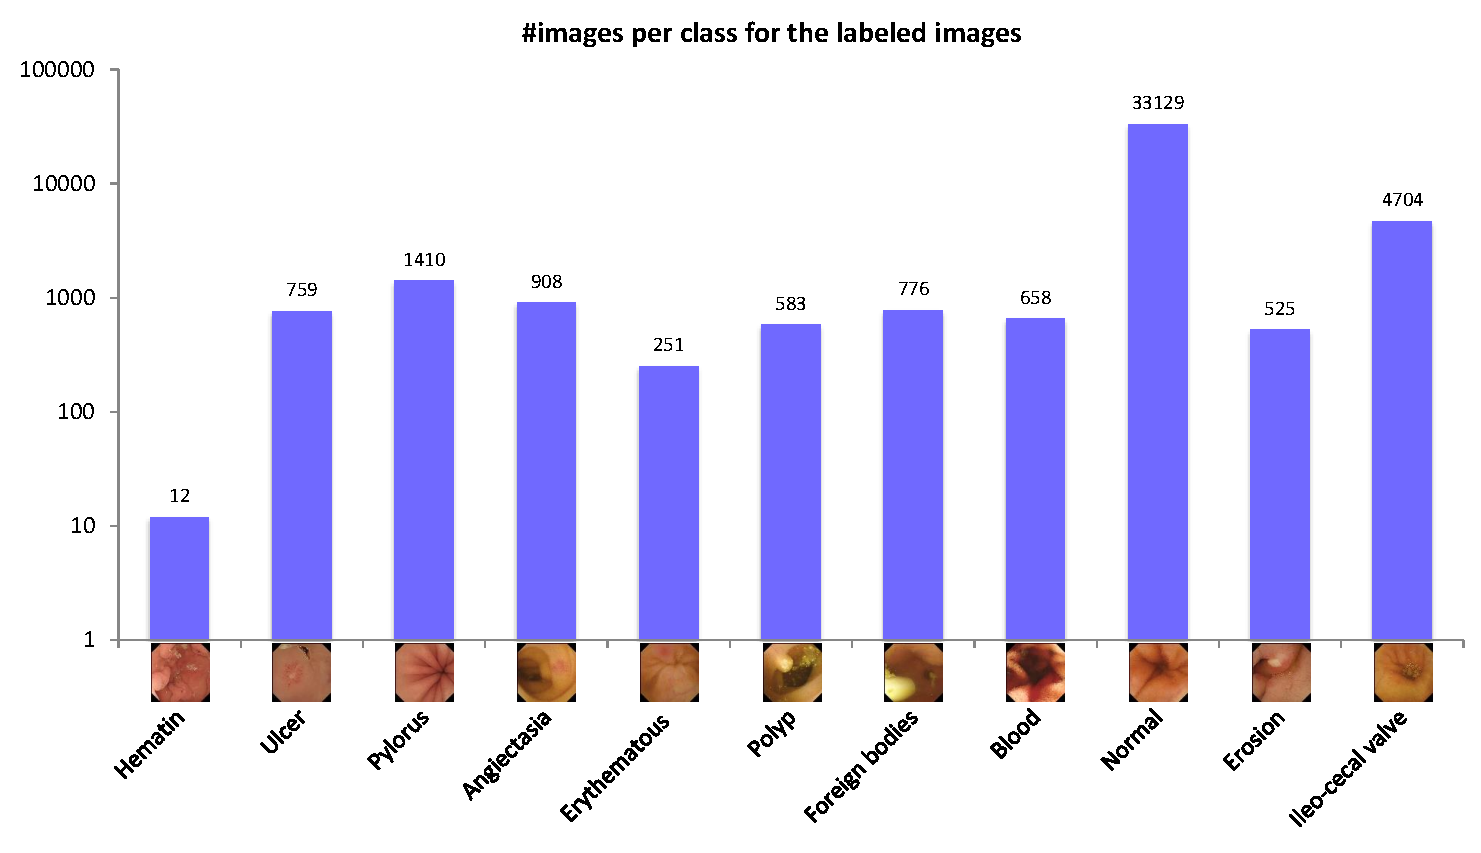
\includegraphics[width=1.0\textwidth]{hyper-capsulecam-dist}
    \caption[Distribution of samples per class in the Hyper-CapsuleCam dataset.]{The distribution of samples per class in the Hyper-CapsuleCam dataset. NB, the Y-axis of this plot is in algorithmic scale.}
    \label{fig:hyper-capsulecam-dist}
  \end{center}
\end{figure}

%TODO : update this table with the final classes and numbers
\begin{table} % table:kvasir_pillcam
  \centering
  \begin{tabular}{|l|r|l|}
  	\hline
  	Class name & \# samples & Percentage \\
    \hline
    Angiectasia		& 908	& xx,x \\ 
    Blood			& 658	& xx,x \\ 
    Erosion			& 525	& xx,x \\ 
    Erythematous	& 251	& xx,x \\
    Foreign Bodies	& 776	& xx,x \\
    Hematin			& 12	& xx,x \\
    Ileo-cecal valve& 4704	& xx,x \\
    Normal			& 33,129& xx,x \\
    Polyp			& 583	& xx,x \\
    Pylorus			& 1410	& xx,x \\
    Ulcer			& 759	& xx,x \\
    Unknown			& 190	& xx,x \\
    \hline
  \end{tabular}
  \caption[Hyper-CapsuleCam class names and number of samples.]{Hyper-CapsuleCam class names, corresponding amount of samples and the percentage of samples in each class.}
  \label{table:kvasir_pillcam_samples}
\end{table}



\subsubsection{Unlabeled images}
Later, we received an additional XX videos. These videos were not annotated but used for unlabeled data. (and/or sample-videos?)
These videos were processed exactly the same as previous videos, so that it will be compatible (**describe**) with the annotated dataset.
%TODO mention number of samples, a rough distribution, image dimensions



\subsubsection{Videos}
In addition to the labeled and unlabeled images all of the videos used for extracting them are included in the dataset in MP4 format. They are weakly labeled by a clinical expert.
%TODO mention the included excel sheet with tags, size of dataset, format, number of frames, etc



% ----------------------------------------------------------
\section{Data pipeline} \label{sec:data_pipeline}
% ----------------------------------------------------------
% Present everything related to working with data files
% tensorflow.data.Dataset pipeline with prefech, batching, shuffling, caching etc
% ----------------------------------------------------------
The preprocessing pipeline is implemented by using TensorFlows \textit{data.Dataset} library. This was chosen over \textit{datagenerator} due to the easy of use, but later became an issue due to the complexity and some diffuse runtime errors. The main benefits by using data.Dataset is that all data is handled in tensors and computation is automatically distributed to the GPU which enhance the load distribution of processing power. In Figure \ref{fig:training_pipeline} is a course look at how our network is trained and the scripts used to do so. The input pipeline sits between the training and test dataset and the TensorFlow model.
%TODO add pointer to the pipeline.py script! and move figure to draw.io

\begin{figure} % fig:training_pipeline
  \begin{center}
    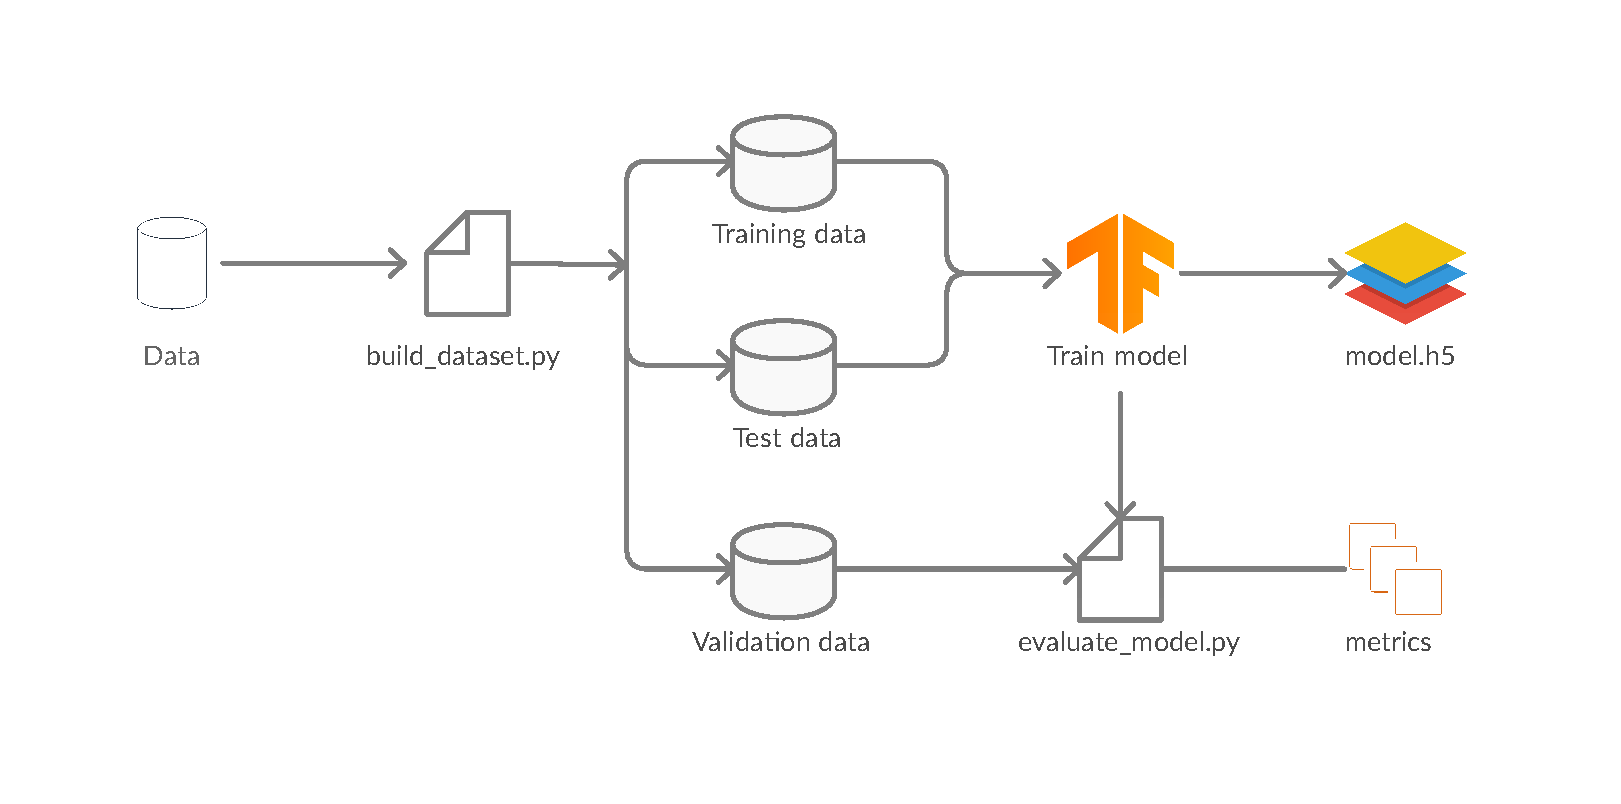
\includegraphics[width=1.0\textwidth]{training_pipeline}
    \caption[Pipeline for training model.]{The pipeline used for training our teacher model.}
    \label{fig:training_pipeline}
  \end{center}
\end{figure}

All the code for handling the data pipeline is managed in a separate script called pipeline.py. The input pipeline outline can be seen in Figure \ref{fig:input_pipeline}.

\begin{figure} % fig:input_pipeline
  \begin{center}
    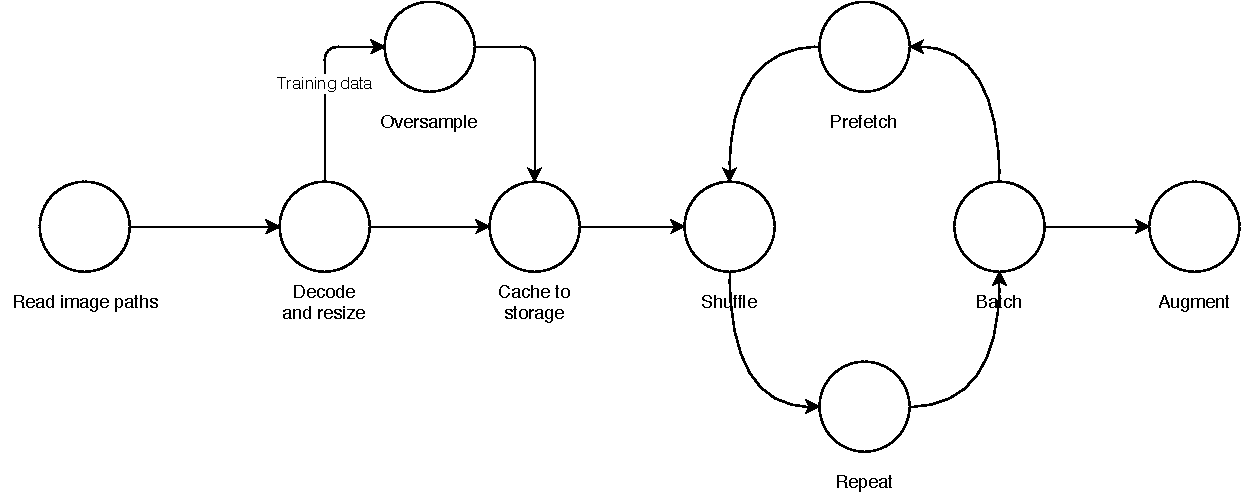
\includegraphics[width=1.0\textwidth]{input_pipeline}
    \caption[The input pipeline]{The input pipeline we use for feeding our network with image-label pairs during training.}
    \label{fig:input_pipeline}
  \end{center}
\end{figure}




\subsection{Splitting and resize images}
% could also be called 'image preprocessing'?
% ----------------------------------------------------------
Although not strictly a part of the pipeline itself the preprocessing is a vital step in machine learning as the quality of the data and the useful information that can be derived from it directly affects the ability of our model to learn.

Initially the dataset was split into three; training data, test data, and validation data. This was done by using tf.data.Dataset core operations \textit{take} and \textit{skip}. The take function, when called upon, returns a sub-dataset with the same number of samples as the number it receives as a argument. Skip function returns a sub-dataset where it skips the number of elements as stated in input argument and return the remaining samples.

\begin{lstlisting}[language=Python]
>>> dataset = tf.data.Dataset.range(10)
>>> dataset = dataset.skip(7)
>>> list(dataset.as_numpy_iterator())
[7, 8, 9]
\end{lstlisting}

However, because of the imbalanced dataset we have been working with this turned out to drop minority classes in some runs. This happened because the take and skip methods picks samples from the entire dataset as whole, and not per class. In Hyper-Kvasir the class with smallest number of samples, called a minority class, is hemorrhoids with 6 samples. Depending on the random shuffling for each run these samples would often all end up in one of the dataset splits and not be represented in the other two.
%Discovered non-optimal implementation of dataset splitting, which left some of the most vulnerable minority classes with no samples in the test data. 
To mitigate this issue I created a separate script for pre-splitting dataset into sub folders for each, training, testing and validation dataset. The outline of this script is given below.

\begin{lstlisting}[language=Python]
for every class name in directories:
	sort the images
	shuffle the filenames
	split the class into train, test and val
	for each split_ds in datasets:
		for filename in sub-split:
			resize and save the image
\end{lstlisting}

We split the data into 60\% training data, and leave 15\% for test data and validation data respectively. To make the split reproducible we first sort the data in alphabetically order after file names then use seeded random to shuffle the filenames so the three datasets contains a random assortment of images from the original dataset. 
In this step we also reduce the image dimensions to 256 by 256 pixels to make the data easier to use during the next preprocessing steps. For downscaling the images we use a \textit{resize} function from the highly optimized library openCV's, with a bilinear interpolation. We used openCV because for this particular task it was about 30\% faster than Pillow, another popular Python imaging library. However this downscaling might introduce aliasing and artifacts to the images as the Hyper-Kvasir's median image dimensions are 768 by 576 pixels, which means we are reducing the dimensions with a factor of three. Area based interpolation \cite{AreaBased99} or Gaussian resampling, with a suitable chosen radius, may give better results. This is something I would like to have tested if I had more time.

Another benefit we get from running all images through this processing script is the reduction in dataset file size. In Hyper-Kvasir this size reduction correspond to a magnitude in total file size reduction, from 28 gigabytes to 2.8 gigabytes. This helps to efficiently load the images into the pipeline during training.

At this step it would be natural to also apply normalization to the images, but TensorFlow handles this gracefully while reading the images from disk, so we have opted to leave this out of the script. To normalize an image in the context of machine learning means to squeeze the pixels values into a range from zero to one. This is done because usually when reading an image from disk it is represented with an integer value between 0 and 255. Although this integer value can be directly represented to the neural network models, this can result in challenges during training like slower learning.

Finally the images are saved to a corresponding directory for each train, test and validation data in the given output directory.



\subsection{Loading images into the pipeline}
% write about the first part of create_dataset script
% ----------------------------------------------------------
To efficiently read and process the images in the pipeline we use TensorFlow's function \textit{list\_files} from the tensorflow.data API. This function creates a Python iterable dataset object of all files matching a glob pattern. An example of a glob pattern could be "/source/datasets/*.jpg". In this example the "*.jpg" is a wildcard followed by a image format extension, which means that a dataset will be created out of all jpg images inside the "datasets" directory. This function then returns a dataset of strings corresponding to filenames. Although not strictly necessary because the images were randomly shuffled before being split into train, test and validation datasets, the filenames are shuffled again upon entering the dataset. This is repeated three times for each of the train, test and validation datasets. If we get 5 samples from this dataset of strings this is how they would be represented:

\begin{lstlisting}[language=Python]
>>> for path in dataset.take(5):
>>> 	print (path)
tf.Tensor(b'/normal-cecum/cc6ed77fbc04.jpg', shape=(), dtype=string)
tf.Tensor(b'/polyps/119100adf1de.jpg', shape=(), dtype=string)
tf.Tensor(b'/esophagitis/f3be6279f5f7.jpg', shape=(), dtype=string)
tf.Tensor(b'/dyed-lifted-polyps/dfb00c142d.jpg', shape=(), dtype=string)
tf.Tensor(b'/dyed-lifted-polyps/aa0268867b.jpg', shape=(), dtype=string)
\end{lstlisting}

Next we apply a transformation function to each element of the dataset to create (image, label) pairs from the filepaths. This transformation function does three things; one-hot encodes the label based on the parent directory; decodes the image so the image is represented with a tensor with dimensions (image width, image height, color channels); resize the image to the correct dimensions. 

Once we have a dataset object we can transform it into a new dataset by chaining method calls on the dataset object.



\subsection{Optimize performance}
%source1: https://www.tensorflow.org/guide/data_performance#optimize_performance
%source2: https://www.tensorflow.org/api_docs/python/tf/data/Dataset#cache
% ----------------------------------------------------------
To build a efficient pipeline it is required that the Graphical Processor Unit (GPU) is fed data at the right time. If the GPU is waiting to receive data the pipeline is not optimized and training will take longer. Preferably the pipeline delivers data for the next step before the current step has finished. 

The main steps involved in training a model is (1); opening a file, (2); reading the data from that file and (3); using the data for training. If these operations are performed in synchronous and sequential order the model can not train while it is waiting idle for an image to be opened and read. Therefore the training step time is the sum of all three steps, see Figure \ref{fig:pipeline_naive}. 

\begin{figure} % fig:pipeline_naive
  \begin{center}
    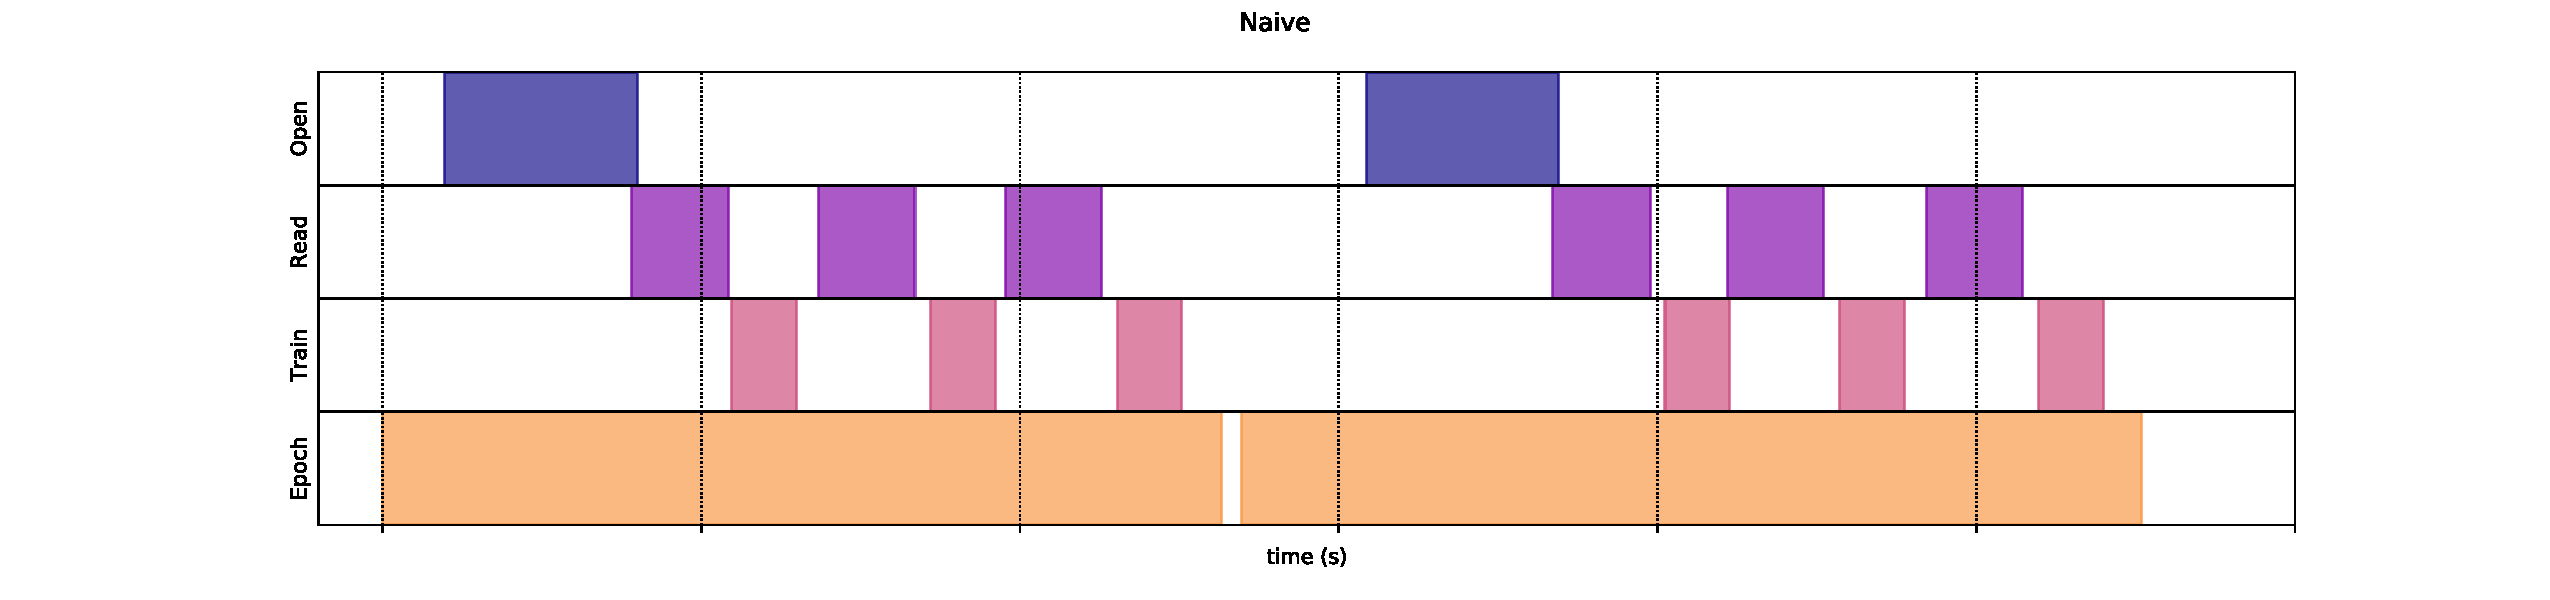
\includegraphics[width=1.0\textwidth]{pipeline_naive}
    \caption[Naive pipeline.]{The time spent for reading, opening and training - the naive method.}
    \label{fig:pipeline_naive}
  \end{center}
\end{figure}

To mitigate this time-consuming issue the tf.data API have a couple of tools at disposal. The first one is prefetching. 
Prefetching overlaps the preprocessing and model execution of a training step. While the model is executing training step $s$, the input pipeline is reading the data for step $s+1$. Doing so reduces the training step time by a significant amount as seen on Figure \ref{fig:pipeline_prefetch}.
Because we are using a tf.data.Dataset object for holding all our images it is very easy to introduce prefetching to the pipeline. The tf.data API provides the tf.data.Dataset.prefetch transformation which decouple the time when data is produced by the CPU from the time when data is consumed by the GPU. 

\begin{figure} % fig:pipeline_prefetch
  \begin{center}
    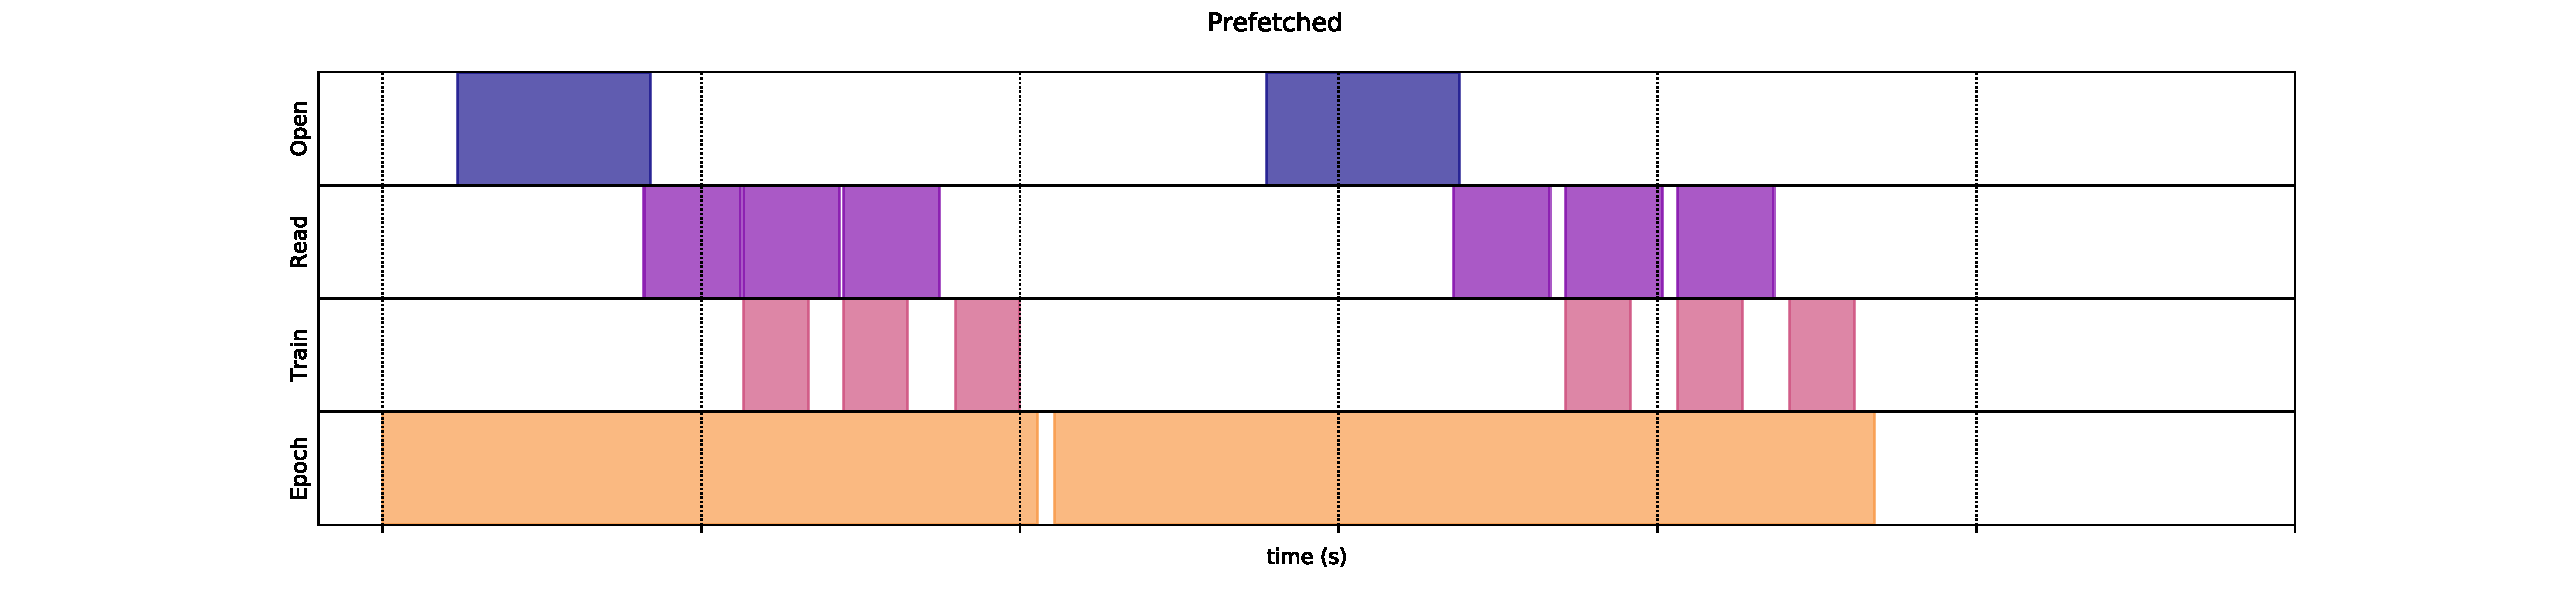
\includegraphics[width=1.0\textwidth]{pipeline_prefetch}
    \caption[Pipeline with prefetching.]{Time spent on reading, opening and training with pipeline prefetching enabled.}
    \label{fig:pipeline_prefetch}
  \end{center}
\end{figure}

We rely heavily on data augmentation to help the model to generalize and not overfit. This is done when preparing the data by using tf.data.Dataset.map transformations, which applies a user-defined function to each element of the input dataset. Because the samples are independent of one another, the process can be parallelized across multiple CPU cores. The tf.data API provides a num\_paralell\_calls argument to specify the level of parallelism, this argument can be set manually or automatically. We have chosen to go with the automatic delegation, which sets the level of parallelism on runtime. See Figure \ref{fig:pipeline_sequential} for the naive approach, and Figure \ref{fig:pipeline_parallel_map} for overhead when using parallel mapping.

\begin{figure} % fig:pipeline_sequential
  \begin{center}
    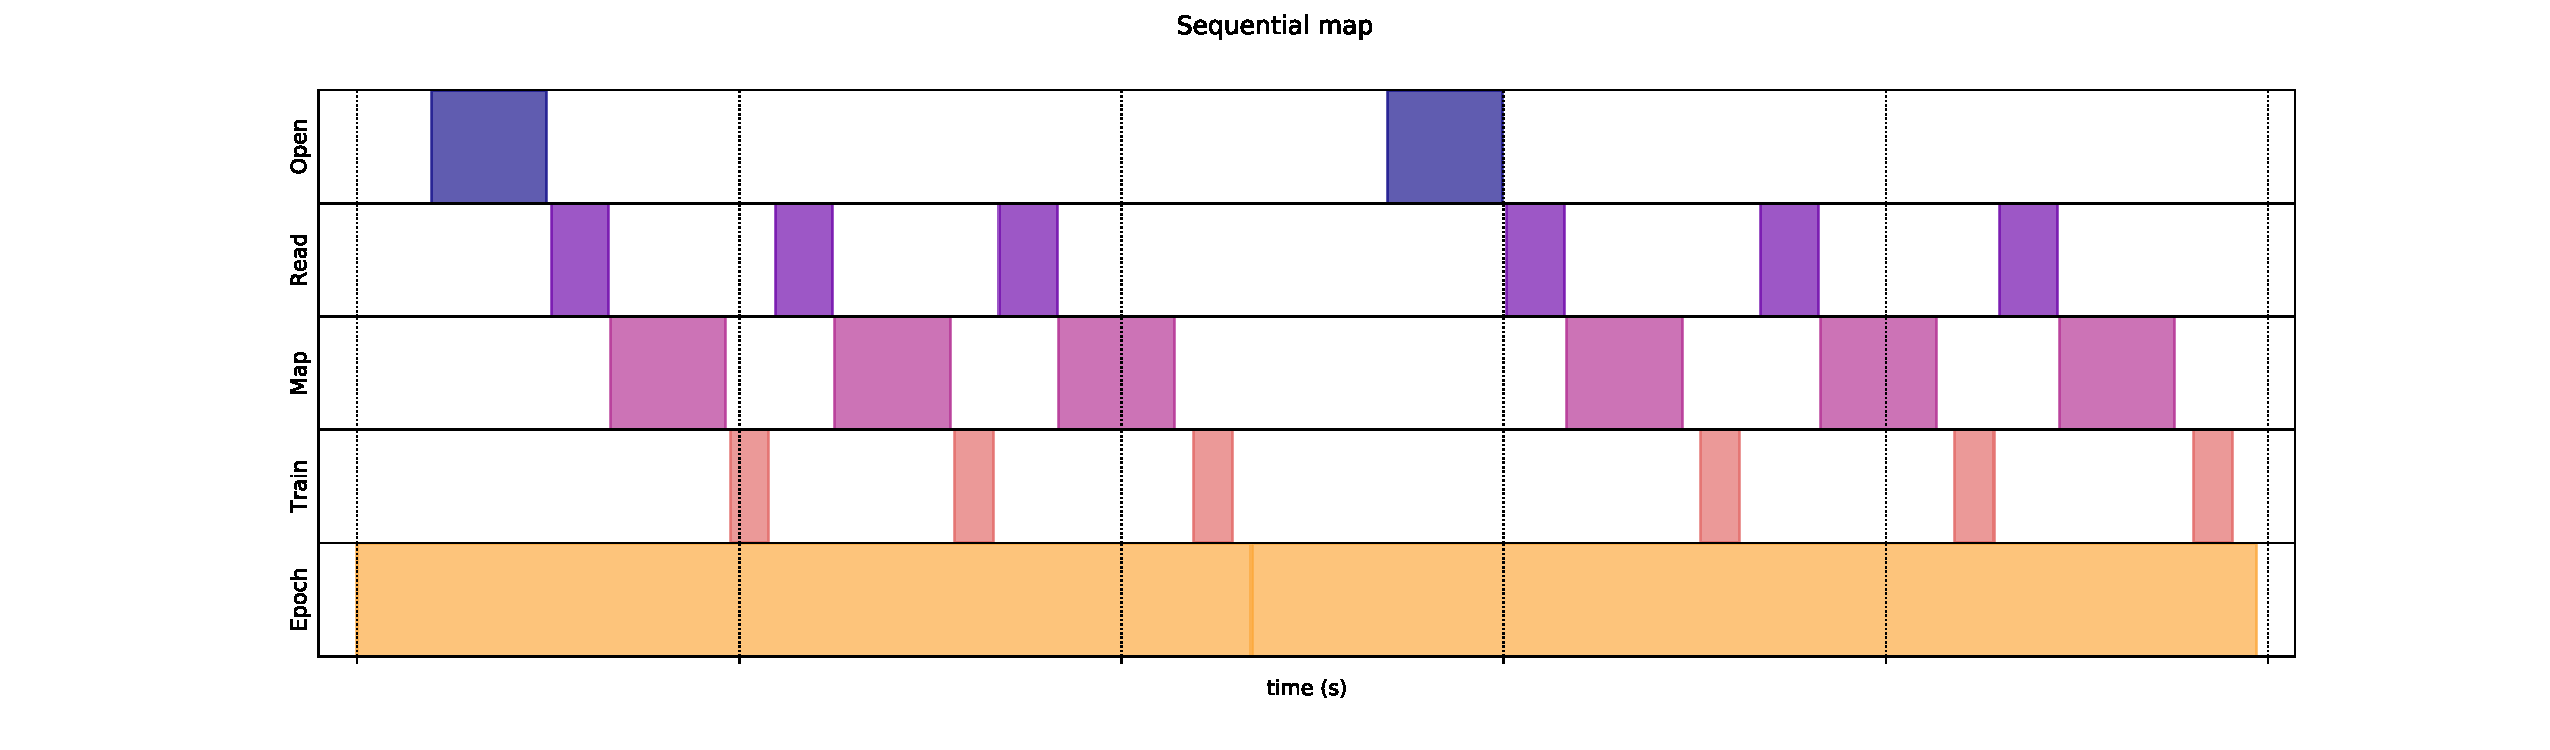
\includegraphics[width=1.0\textwidth]{pipeline_sequential}
    \caption[Naive pipeline with mapping.]{Naive pipeline, here the times spent on opening, reading, pre-processing and training steps sum together for a single iteration.}
    \label{fig:pipeline_sequential}
  \end{center}
\end{figure}

\begin{figure} % fig:pipeline_parallel_map
  \begin{center}
    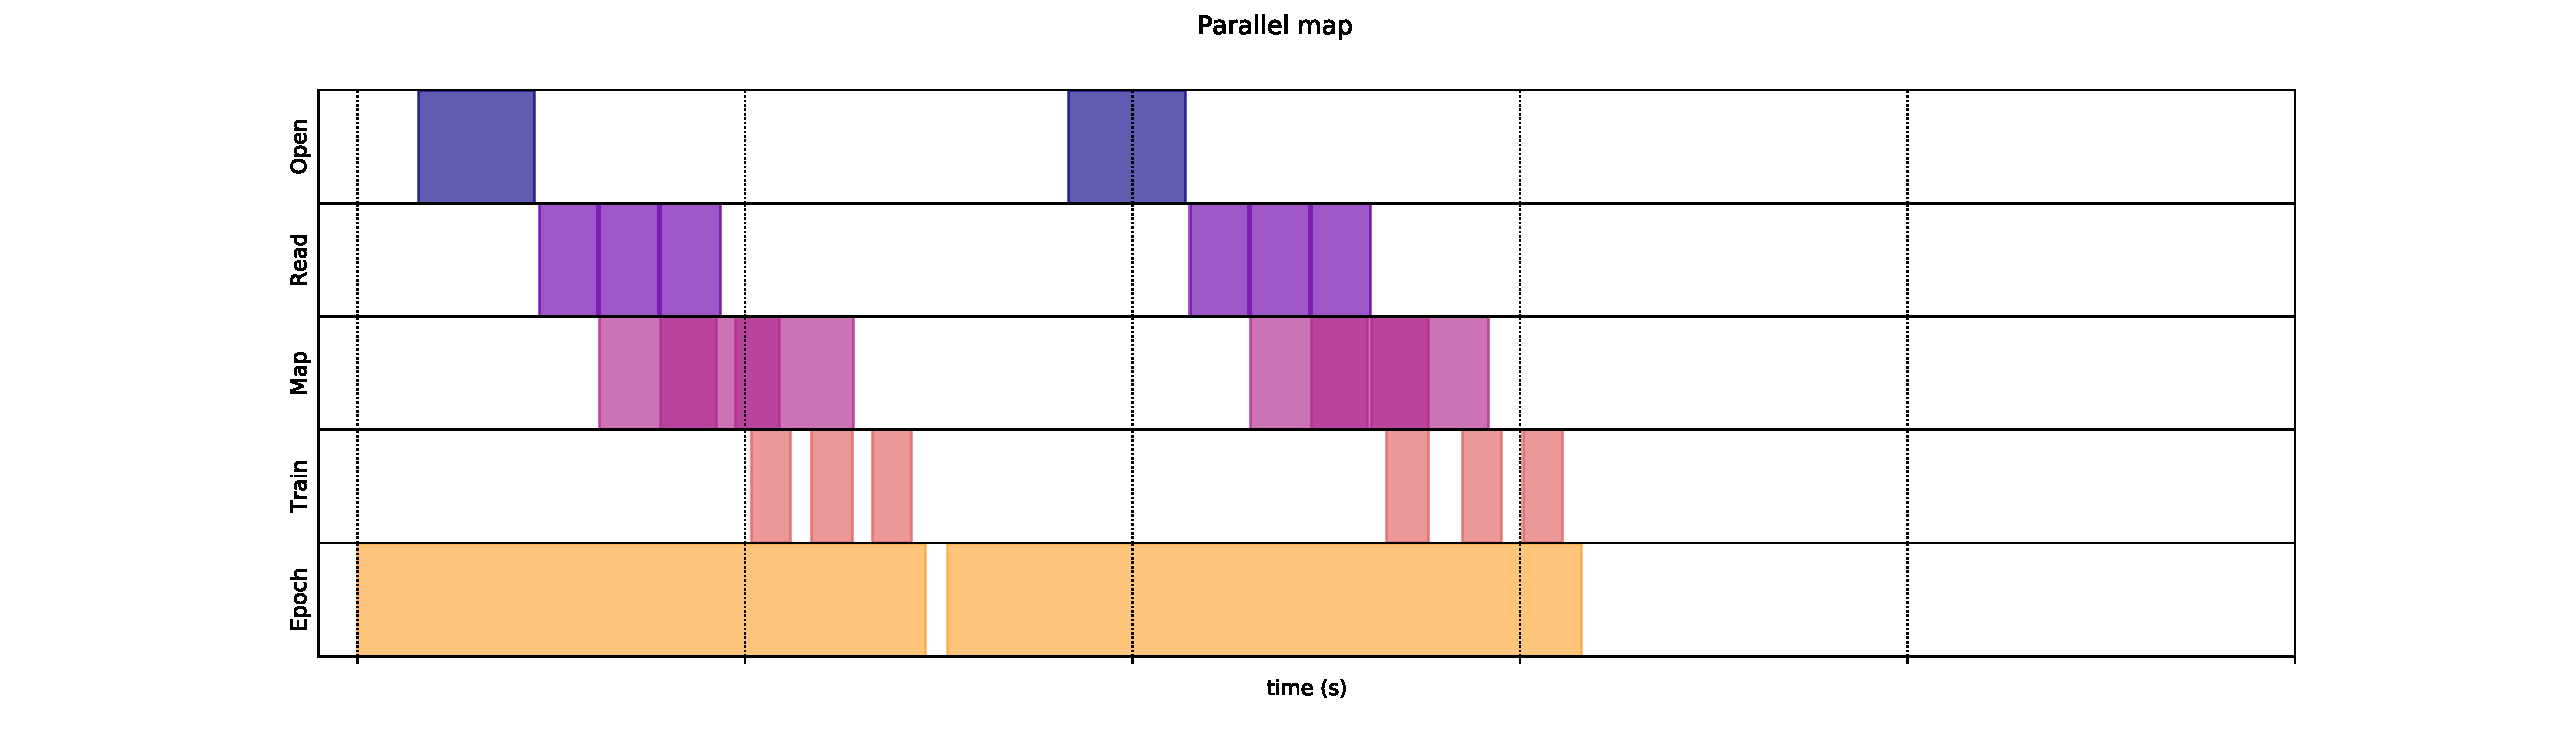
\includegraphics[width=1.0\textwidth]{pipeline_parallel_map}
    \caption[Pipeline with parallel mapping.]{Here you can see pre-processing steps overlap, and the overall time for each iteration is reduced.}
    \label{fig:pipeline_parallel_map}
  \end{center}
\end{figure}

The last step we take to optimize the training efficiency is to cache the dataset to local storage (an NVMe SSD in our case). This will save some operations, like opening and reading data, from being executed each epoch during training of the model. 
When the dataset is cached, the images will be opened, read and in our case some pre-processing are performed, the first epoch during training, and the following epochs will reuse the data stored in the local cache. See Figure \ref{fig:pipeline_cache} for an example of how this affects time consumption.
We split the pre-processing steps into two steps. The first step is applied before caching the dataset and the last step is performed after. This is done because some pre-processing steps are to be performed on every element of the dataset in a deliberate way, and some steps are randomized every time the process is applied.
The mapping that are applied before the caching is: read the label and one-hot encode to integer, read and decode the image, normalize image and resize image dimensions. The mappings that are performed after caching is: shuffling, batching, augmenting.

\begin{figure} % fig:pipeline_cache
  \begin{center}
    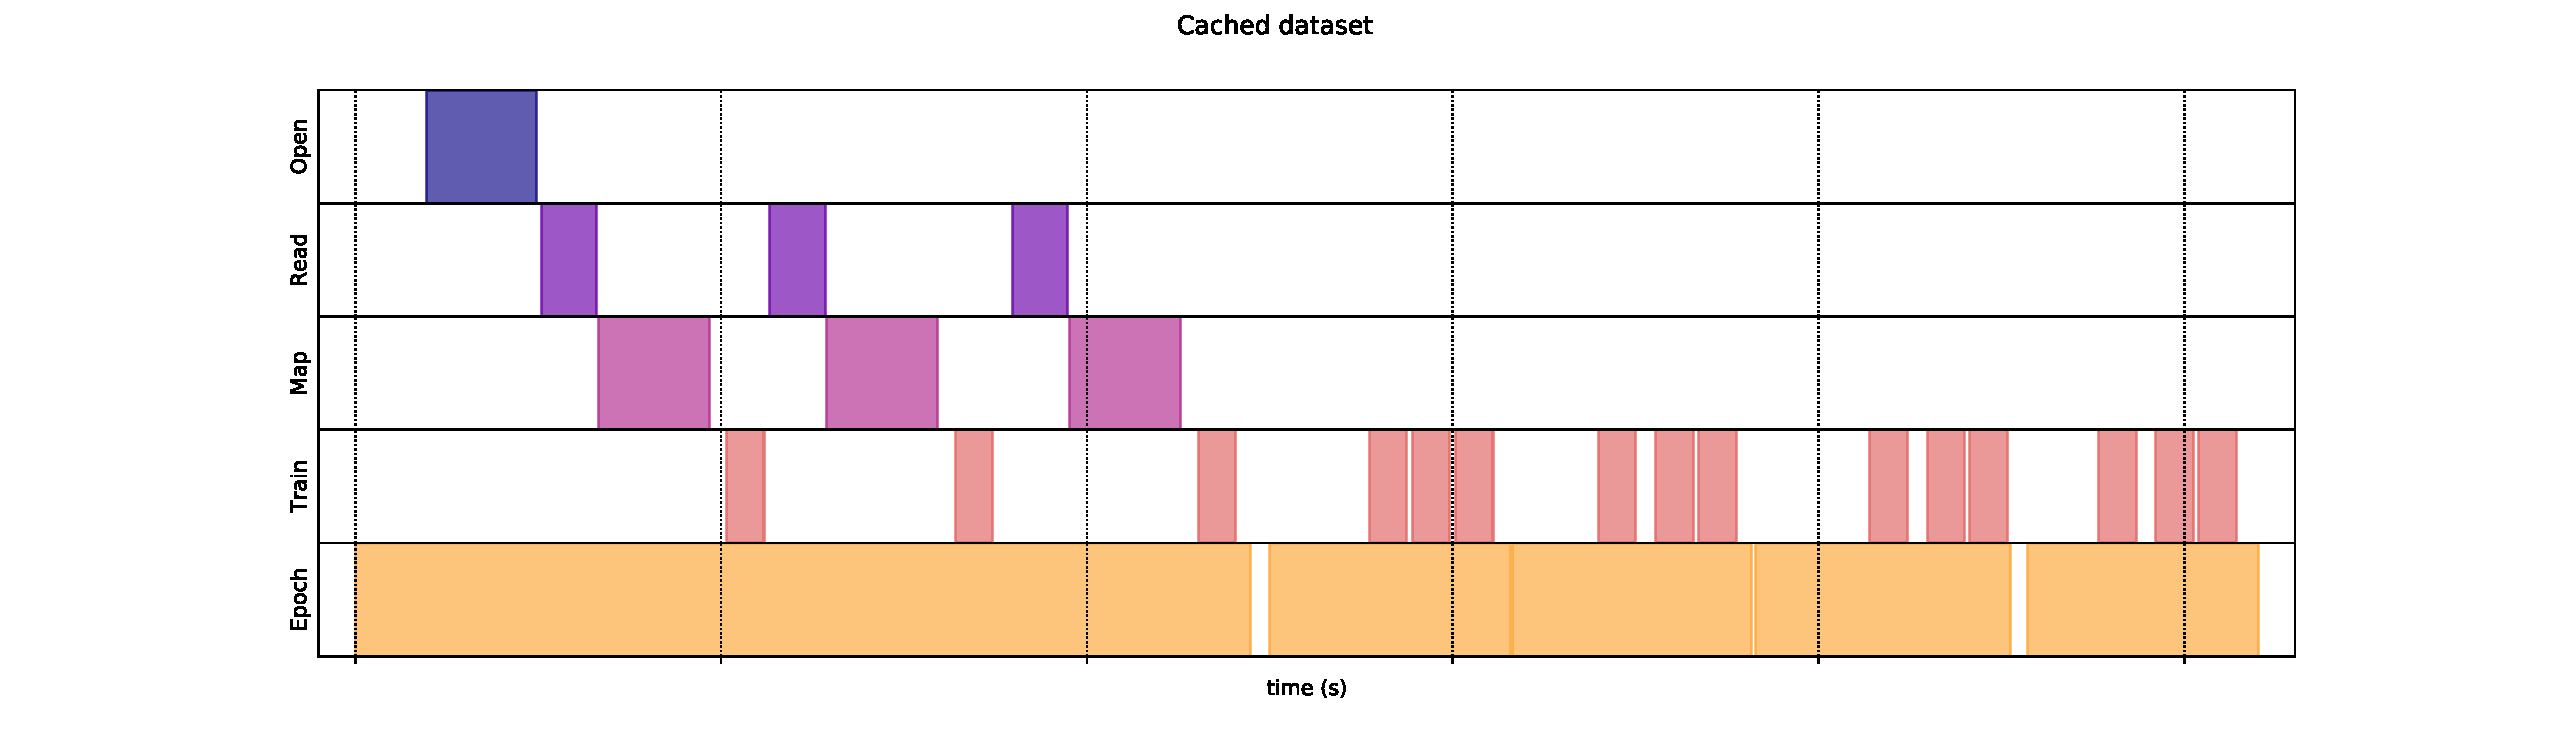
\includegraphics[width=1.0\textwidth]{pipeline_cache}
    \caption[Pipeline with cache.]{Cached pipeline, here the pre-processing is only executed during the first training step.}
    \label{fig:pipeline_cache}
  \end{center}
\end{figure}



\subsection{Shuffle the dataset}
% source tf: https://www.tensorflow.org/api_docs/python/tf/data/Dataset#shuffle
% ----------------------------------------------------------
We shuffle the data to reduce variance and to make sure the model remain general and overfit less. This is especially important as our dataset is sorted by their classes.
In our pipeline the data is shuffled twice for redundancy. We can afford this because the tf.data API has a low computational performance hit the way it applies the shuffle transformation. 
The pipeline shuffles the entire list of image filepaths initially, and then a shuffle transformation is applied a second time after the dataset is cached, this ensure that the dataset is shuffled between every epoch during training as well. This is important because we have the risk of creating batches that are not representative of the overall dataset, and therefore gradient estimate will be off.

TensorFlows data API have a dedicated shuffle function which randomly shuffles the elements of the input dataset. It does this by filling a buffer of $n$ elements, then randomly sample elements from this buffer, replacing the selected elements with new elements. For perfect shuffling of the entire dataset we use $n>$ \textit{total\_samples}. The argument \textit{reshuffle\_each\_iteration} is set to \textit{True} so every epoch get an unique batch of images.

Another method of creating unique batches is to first repeat the dataset, then shuffle and create batches.



\subsection{Repeat}
% is the data always repeated? how resampling effect this?
% ----------------------------------------------------------
In some situations it is desirable to extend the dataset with duplicates of past samples. One example of this is for oversampling the dataset. 
We use the \textit{repeat} function from the tf.data API to "infinitely" repeat the dataset samples.

\begin{lstlisting}[language=Python]
>>dataset = tf.data.Dataset.from_tensor_slices([1, 2, 3])
>>dataset = dataset.repeat()
>>list(dataset.as_numpy_iterator())
[1, 2, 3, 1, 2, 3, 1, 2, 3, .....]
\end{lstlisting}

This repeat transformation is applied after caching and shuffling, so that we are sure the model sees every sample of the dataset each epoch. We then apply image augmentation at random to each dataset sample so for every finished epoch during training every image is shown once, with a distinctive augmentation filter.

Because the dataset is infinitely repeated we must specify how many steps the model should iterate during training, or else it would not know where to stop iterating through the dataset object.



\subsection{Data augmentation}
% https://www.kdnuggets.com/2020/02/easy-image-dataset-augmentation-tensorflow.html
% What is the necessity of rotating the samples. Will they not always be 'square'?
% ----------------------------------------------------------
The datasets we will be performing our experiments on, like many medical domain datasets, share a common unbalanced data problem. That is images of the target classes, only appear in a very small portion of the the entire dataset. 

Having a large amount of labeled images is important for the performance of all medical image classification models to effectively learn. Data augmentation overcomes this issue by artificially inflating the training set with label preserving transformations. This helps the model to generalize better and to overfit less - overall a more robust model.

This augmented data is acquired by performing a series of pre-processing transformations to existing data. These transformations can include horizontal and vertical flipping of the image, skewing, cropping, rotating and much more. By doing this, the augmented data is able to simulate a variety of subtly different data points, as opposed to just duplicating the same data over and over. In Figure \ref{fig:data_aug-crop-rot} we have taken one Image from the Hyper-Kvasir dataset and created a tf.data.Dataset object which has then been repeated and gone through the same data augmentations that we use in the input pipeline for the training data.

\begin{figure} % fig:data_aug-crop-rot
  \begin{center}
    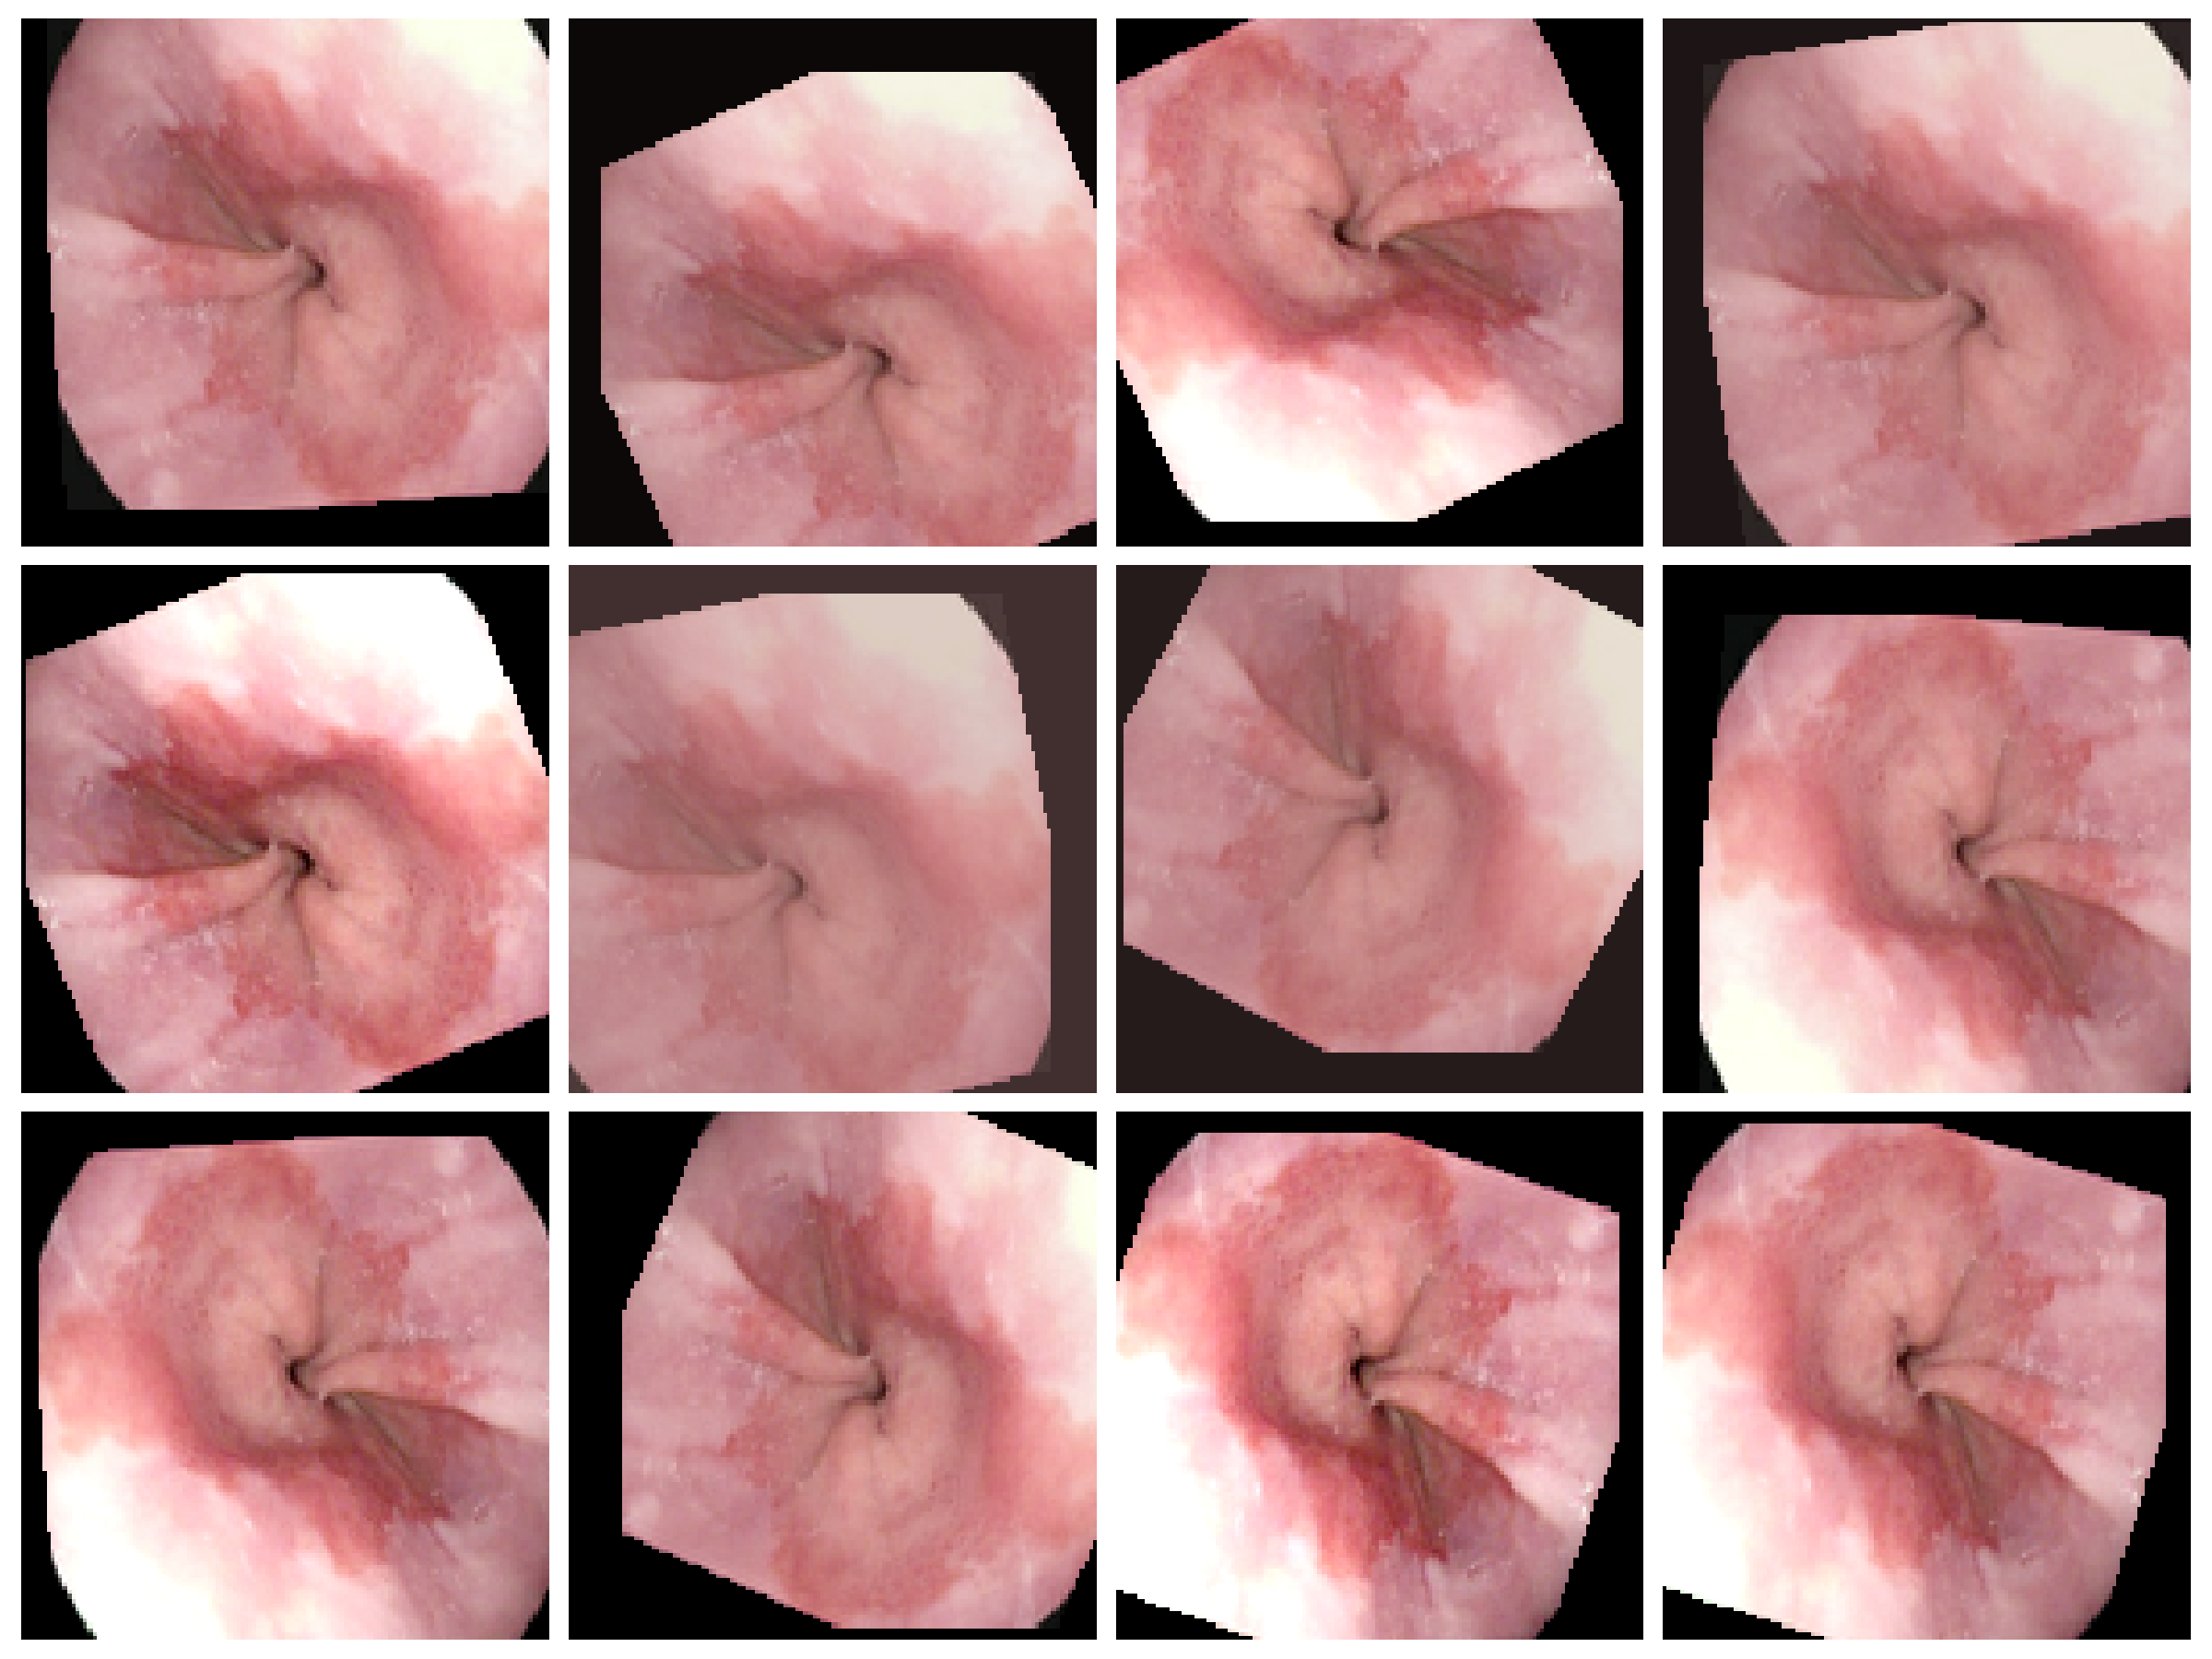
\includegraphics[width=.7\textwidth]{data_aug-crop-rot}
    \caption[The effect of data augmentation on sample image.]{The effect of data augmentation on an image from Hyper-Kvasir. Image taken from barrets-short-segment class.}
    \label{fig:data_aug-crop-rot}
  \end{center}
\end{figure}

This is especially important in the medical domain of VCE videos due to two reasons; (1), the camera capsule will orient itself randomly as it travels through the small intestine, and the model have to able to detect a polyp regardless of the orientation and (2), we have a very uneven class balance within the dataset and oversample the minority classes requires some sort of data augmentation to reduce overfitting.

Data augmentation will however not solve all data problems, but it has been proven to be very effective for training neural networks. By implementing data augmentation in our pipeline we saw that during training the model would overfit far less. The augmentation transformation we use is as follow:

\begin{itemize}
\item \textbf{Flip}; mirroring the images across its vertical or horizontal axis. It is computationally efficient and easy to implement as it only requires rows or columns of image matrices to be reversed.
\item \textbf{Rotation}; rotates the image around its center via mapping each pixel $(x,y)$ of an image to $(x',y')$ with the following transformation
	\[ \begin{pmatrix} x' \\ y' \end{pmatrix} =
	\begin{pmatrix} cos \theta & -sin \theta \\ sin \theta & cos \theta \end{pmatrix}
	\begin{pmatrix} x \\ y \end{pmatrix} \]
We find that setting $\theta$ to a random number between $-30$ degrees and $+30$ degrees give good results.
\item \textbf{Crop}; pad the image by adding black pixels around the image and then randomly crop it back down to the original image dimensions. We have chosen that the image is padded with 20\% of its original dimensions. For example a image with the dimensions 128 by 128 will be padded with 25 pixels.
\item \textbf{Brightness}; convert RGB image to float representation, adjusts the brightness, and then convert the image back to original data type. We have set a value, $max\_delta=0.25$, and randomly pick a value from the interval [-max\_delta, max\_delta] which is the amount to add to the pixel values.
\item \textbf{Saturation}; converts the image to HSV, adds an offset to the saturation channel and then converts the image back to RGB. The offset is randomly selected from the interval [lower, upper]. In our experiments we have set the interval to [0.6, 1.5].
\item \textbf{Contrast}; converts images to float representation, adjusts their contrast, and then converts them back to the original data type. Contrast is adjusted independently for each channel of each image. This is done by computing the mean of the image pixels for each channel and then adjusts component $x$ of each pixel to $(x-mean)*contrast\_factor+mean$. Where contrast\_factor is randomly picked from the interval [lower, upper] $=[0.6, 1.5]$.
\end{itemize}

To selectively choose how much the dataset is augmented during training of a model we have implemented a system which dial back the aforementioned parameters by a percentage. This enables us to train the teacher model with very little augmentation and then increase the image augmentations for the student model. In Figure \ref{fig:data_aug-reduced} is an example of a batch of 12 images which is shown to the network during training.

One possible draw-back from using data augmentation is the network might miss important features during training if those features are cropped or rotated out of view. With this in mind we use cropping and rotation with care. For cropping we dial back the padding to just 10\% and rotation is dialed back to only 10 degrees rotation at most.
% include discussion part form "Data augmentation for improving deep learning in image classification problem"?

\begin{figure} % fig:data_aug-reduced
  \begin{center}
    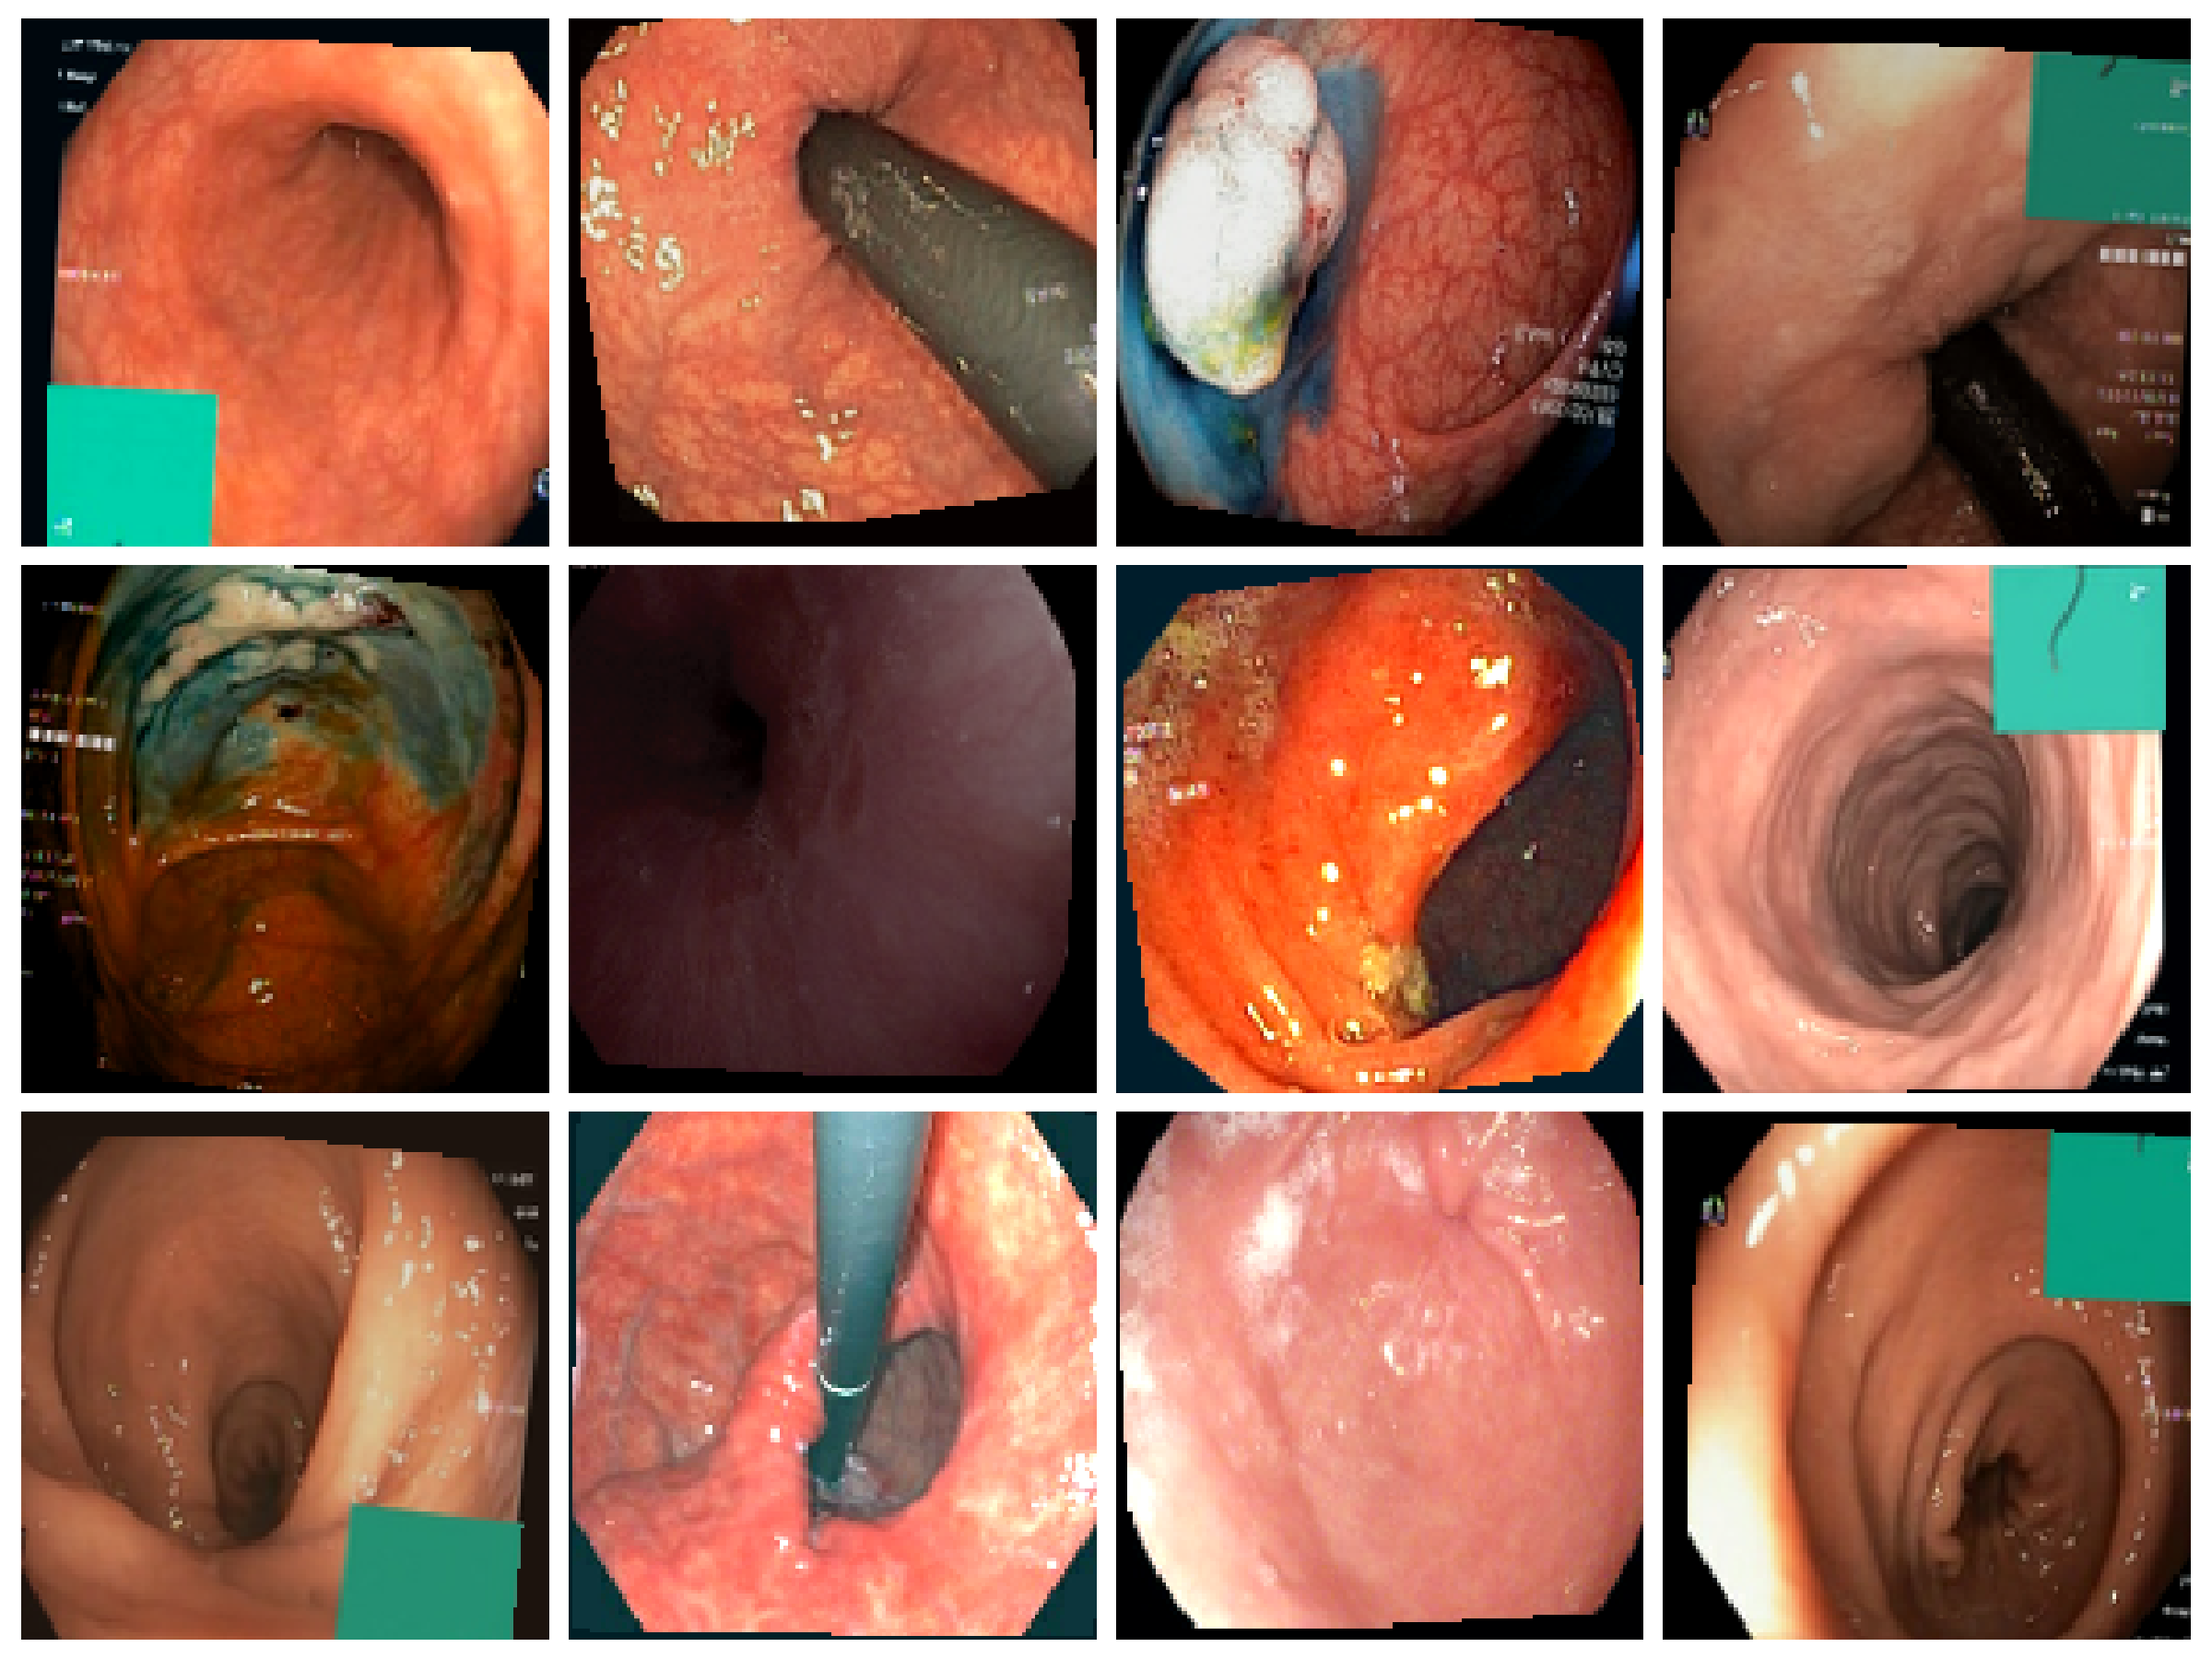
\includegraphics[width=.7\textwidth]{data_aug-reduced}
    \caption[The effect of reduced data augmentation on sample image.]{The effect of reduced data augmentation on images from Hyper-Kvasir dataset. Here the effect of cropping is reduced by padding the image with 10\% of its original dimensions, and rotation is reduced to max 10 degrees.}
    \label{fig:data_aug-reduced}
  \end{center}
\end{figure}

In recent years, automated augmentation strategies have led to state-of-the-art results in image classification and object detection \cite{AutoAugmentLearning19, RandAugmentPractical19}. These novel automated augmentation policies have shown to improve accuracy, model robustness, and performance on semi-supervised learning for image classification without no additional computational cost at inference time. Due to time constraint we did not test this on our network, but is something we would like to implement in future studies.



\subsubsection{tf.image}
% https://www.tensorflow.org/api_docs/python/tf/image
We have used tf.image API from TensorFlow for all our data augmentations within the input pipeline. This module contains functions for image processing and decoding-encoding operations, and use little computational overhead. All functions that select a random value from an interval have the option to be seeded so that our data is reproducible.



\subsection{Batching}
% https://www.tensorflow.org/api_docs/python/tf/data/Dataset#batch
% https://machinelearningmastery.com/how-to-control-the-speed-and-stability-of-training-neural-networks-with-gradient-descent-batch-size/
% ----------------------------------------------------------
% Why is batching useful
The batch size is a hyperparameter that defines the number of samples to work through before updating the internal model parameters. At the end of each batch, the image predictions are compared to the expected output of the model and an error is calculated. The update algorithm use that error to improve the model, e.g move down along the error gradient.
In the domain of machine learning is is common to name the learning algorithm based on three criterion:
\begin{itemize}
\item \textbf{Batch Gradient Descent}: all training samples are used to create one batch.
\item \textbf{Stochastic Gradient Descent}: batch size is one element of the training data.
\item \textbf{Mini-Batch Gradient Descent}: batch size is more than one sample and less than the size of the entire dataset
\end{itemize}

% How do we batch
Like with the rest of the operations performed in the input pipeline, TensorFlow tf.data API have its own module for batching a dataset. This module have two parameters, one for batch size, and the other for whether the last batch should be dropped in the case it has fewer elements than set by the first parameter. Since our input pipeline repeats the dataset we never run into the issue of having batches which are truncated, so we set this to False.

% Example of tf.data API .batch()
\begin{lstlisting}[language=Python, caption={Notice how \text{[6, 7]} is missing because drop\_remainder is set to True.}, captionpos=b]
>>>dataset = tf.data.Dataset.range(8)
>>>dataset = dataset.batch(3, drop_remainder=True)
>>>list(dataset.as_numpy_iterator())
[array([0, 1, 2]), array([3, 4, 5])]
\end{lstlisting}

% What batch size do we use   - Smaller batch sizes are noisy, offering a regularizing effect and lower generalization error
One advantage of using mini-batch gradient descent is that it requires less memory. In our case the complete dataset will not fit in memory regardless so batch gradient descent is not possible to test. Another advantage is that typically networks train faster, achieves better training stability and generalization performance with mini-batches \cite{RevisitingSmall18}. \citeauthor{RevisitingSmall18} found that when experimenting with different batch sizes on ImageNet, CIFAR-10 and CIFAR-100, batch sizes of 32 or less provides more up-to-date gradient calculations, which yields more stable and reliable training. Other scientific papers also support that batch size of 32 is a good choice \cite{PracticalRecommendations12, GeneralInefficiency03}.
We find that the limiting factor for setting the batch size is GPU memory, especially for larger models like EfficientNetsB2-B7. All models are trained on NVIDIA GTX 1080 ti with 11GB of memory, which can endure at most 64 images with dimensions of 256 by 256 being trained on EfficientNetB0 which has 5.3 million parameters.



\subsection{Dealing with class imbalance}
% remember to mention what changes in caching and shuffling
% ----------------------------------------------------------
To combat the class imbalance in our dataset we have experimented with two tactics. The first thing we tested, which was also the easiest to implement with TensorFlow was class weighting. Weighting the classes means that we calculate a score for every class within the dataset, and during training of the network each classes weight is carried when computing the loss. Normally each class has a weight of 1, but we don't want this because of the nature of class imbalance. Instead, if there are twice as many samples in class A than in class B, we give class A a weight score which is half that of class B.
% what happenes if we dont balance dataset?



\subsubsection{Oversample}
Oversampling the training dataset is handled by a oversample() module inside pipeline.py. This module takes the training dataset as input parameter and then split the dataset into as many separate datasets as there are classes. Because the dataset is stored in a tf.data.Dataset object this must be done according to the tf.data API. We use a transformation method which filters out all image, sample pairs not belonging to the according class. Doing so gives us a python list of one dataset object for each class, containing as many samples as there were originally. The next step is to chache this list of datasets to reduce computational strain when we later want to iterate over the dataset again. Lastly we repeat every dataset so for each class in the list there is infinitely repeating samples. 
TensorFlow has a convenient function for interleaving elements at random from a list of datasets which we use to go from having a list of repeating datasets to one datasets which produces a uniform distribution of randomly picked image, label pairs when iterated over.

\begin{lstlisting}[language=Python]
datasets = []
for i in range(num_classes):
    # Get all samples from class i [0 -> num_classes], repeat the dataset
    # indefinitely and store in datasets list
    data = ds.filter(lambda img, lab: lab==i)
    data = data.cache(cache_dir+'{}_ds'.format(i))
    data = data.repeat()
    datasets.append(data)
    
target_dist = [ 1.0/num_classes ] * num_classes
balanced_ds = tf.data.experimental.sample_from_datasets(
    datasets, target_dist, seed=conf["seed"]
)
\end{lstlisting}

When we run this on Hyper-Kvasir dataset we get the following output. Here we see that the classes are highly unbalanced. The class with least samples is hemorrhoids with a ratio of $0.00054$ samples, while the class bbps-2-3 have a ratio of $0.10773$, that is on a order of two magnitudes more samples. The output from after the oversampling shows that all classes have, almost, the same distribution of $\frac{1}{23}=0.04348$.

\begin{lstlisting}[language=Python]
---- Ratios before resampling ---- 
[0.00496378 0.07163939 0.00321975 0.01247652 0.02441642 0.09283606
 0.00053662 0.08746982 0.03783204 0.00093909 0.00375637 0.10772739
 0.00080494 0.06063858 0.01220821 0.09471425 0.04158841 0.00254897
 0.09377515 0.03662463 0.01878186 0.09645828 0.09404346]

---- Ratios after resampling ----
[0.04111328 0.04501953 0.04589844 0.04414063 0.04443359 0.04189453
 0.04033203 0.03916015 0.04453125 0.04619141 0.04091797 0.04628906
 0.04345703 0.04160156 0.04453125 0.04296875 0.04580078 0.040625
 0.04560547 0.04404297 0.04238281 0.04257812 0.04648437]
\end{lstlisting}




\subsubsection{Class weights}
The way we calculate the class weights for our data is by the following formula.

% pythonic: n_samples / (n_classes * np.bincount(y))
\[
w_j = \frac{n}{kn_j}
\]
where $w_j$ is the weight to class $j$, $n$ is the number of observations, $n_j$ is the number of observations in class $j$, and $k$ is the total number of classes.

In tf.Keras we can then give the class weights as a dictionary to the model.fit function like this:

\begin{lstlisting}[language=Python]
class_weights = {"class A": 0.5,
				 "class B": 0.25}
				 
model.fit(train_ds, epochs=10, batch_size=32, class_weight=class_weight)
\end{lstlisting}

What we are doing here is to tell Keras that class A should hold 50\% of the weight for the loss function since it is more important than class B which we accordingly set to 25\%.

In the case of Hyper-Kvasir dataset the class weights we use for our experiments are given in Table \ref{table:class_weights}.

\begin{table} % table:class_weights
  \centering
  \begin{tabular}{rr}
	\hline
   Class &   Weight \\
	\hline
       0 &  8.75911 \\
       1 &  1.0     \\
       2 & 13.5036  \\
       3 &  3.48481 \\
       4 &  1.7807  \\
       5 &  1.0     \\
       6 & 81.0217  \\
       7 &  1.0     \\
       8 &  1.14924 \\
       9 & 46.2981  \\
      10 & 11.5745  \\
      11 &  1.0     \\
	\hline
  \end{tabular}
  \quad
  % table 2
  \begin{tabular}{rr}
	\hline
   Class &   Weight \\
	\hline
      12 & 54.0145  \\
      13 &  1.0     \\
      14 &  3.5614  \\
      15 &  1.0     \\
      16 &  1.04544 \\
      17 & 17.0572  \\
      18 &  1.0     \\
      19 &  1.18713 \\
      20 &  2.31491 \\
      21 &  1.0     \\
      22 &  1.0     \\
      & \\
	\hline
  \end{tabular}
  \caption[Hyper-Kvasir class weights]{Hyper-Kvasir class weights. All weigts below 1.0 are set to a minimum of 1.}
  \label{table:class_weights}
\end{table}

\begin{lstlisting}[language=Python]
---- Class weights ----
{0: 8.759107, 1: 1.0, 2: 13.503623, 3: 3.484806, 4: 1.7806976, 5: 1.0, 6: 81.021736, 7: 1.0, 8: 1.1492445, 9: 46.298138, 10: 11.574534, 11: 1.0, 12: 54.014492, 13: 1.0, 14: 3.5613952, 15: 1.0, 16: 1.0454417, 17: 17.057209, 18: 1.0, 19: 1.1871318, 20: 2.3149068, 21: 1.0, 22: 1.0}
\end{lstlisting}

Notice how the minimum range for class weights are set to 1.0. This is done to stabilize the loss. **find reference and reason**
Found that when weighting the classes the model learns slower. Which means decay rate of learning rate must be lowered for it not to drop too soon. Also increase the buffer for early stopping of training.
%TODO add formula for calculating class weights



\subsection{Training}
%TODO Include a table of computer hardware used for training, and versions of all libraries used (like hicks p.73
% Normalization; any benefit of using L2 normalization in last dense layer when using a pre-defined model?
% ----------------------------------------------------------

\begin{table} % table:system_specs
  \centering
  \renewcommand{\arraystretch}{1.3}
  \begin{tabular}{|c|c|c|c|}
  \hline
  Level		& Category		& Name		& Version \\
  \hline
  \multirow{3}{*}{Hardware} & GPU & Nvidia GTX 1080 ti & \\
  \cline{2-4}
  & CPU & Intel i7-8700K 3.7GHz & \\
  \cline{2-4}
  & Memory & G.SKill 3200MHz 32GB & \\
  \hline
  \multirow{6}{*}{Software} & Operating System & Ubuntu Focal Fossa & 20.04 \\
  \cline{2-4}
  & \multirow{5}{*}{Library} & Python & 3.7.6 \\
  \cline{3-4}
  & & TensorFlow & 2.1.0 \\
  \cline{3-4}
  & & Keras & 2.3.1 \\
  \cline{3-4}
  & & Cuda & 10.1.243 \\
  \cline{3-4}
  & & cuDNN & 7.6.5 \\
  \hline
  \end{tabular}
  \caption[System specifications]{A table showing the system specifications for the machine used for all training and evaluation sessions.}
  \label{table:system_specs}
\end{table}

% Batch size for each model
Due to memory limitations we are forced to reduce the batch size when training with larger models. If we run with a too large batch size the model will not fit in memory and we get a Out of Memory error (OOM Error). In Table \ref{table:model_bs} is a overview of what batch sizes we are using for which models during training.

\begin{table} % table:model_bs
  \centering
  \begin{tabular}{|c|cc|cc|}
	\hline
	\multirow{2}{*}{Model} & \multicolumn{2}{c|}{128x128} & \multicolumn{2}{c|}{256x256} \\
	\cline{2-5}
	& Batch Size & Time [s] & Batch Size & Time [s] \\
	\hline
	EfficientNetB0 & 256 & 15 	& 64  & 61  \\
	EfficientNetB1 & 128 & 21	& 32  & 91  \\
	EfficientNetB2 & 128 & 22	& 32  & 98  \\
 	EfficientNetB3 & 128 & 28	& 32  & 113 \\
  	EfficientNetB4 & 64  & 38	& 16  & 153 \\
  	EfficientNetB5 & 64  & 52	& 16  & 206 \\
  	EfficientNetB6 & 32  & 72	& 8   & 288 \\
  	EfficientNetB7 & 32  & 95	& 8   & 400 \\
  	\hline
  \end{tabular}
  \caption[Max batch size for each EfficientNet model]{Max batch size used for each EfficientNet model with image dimensions 128 by 128 and 256 by 256 respectively.}
  \label{table:model_bs}
\end{table}



% ----------------------------------------------------------
\section{System implementation} \label{sec:system_implementation}
% ----------------------------------------------------------
% Present the system architecture, some results perhaps
% ----------------------------------------------------------



\subsection{Keeping track of experiemnts}
% write about logging etc
% ----------------------------------------------------------




\subsection{Training the teacher model}
% ----------------------------------------------------------







\subsection{Generating new pseudo labels}
% ----------------------------------------------------------
When we use the trained teacher model to generate new pseudo labels from the dataset we set a threshold for which the predicted image is saved if it is above the set value. Here we have two options, either to set the threshold low and extract a large dataset with high uncertainty, but get the most of our minority classes. Or we can set the threshold high, and gather a dataset with lower uncertainty, but might miss more samples for the minority classes.

After subtracting samples from the unlabeled dataset through predicting and saving images with a probability score higher than the threshold, we sort the images based on the probability scores. This is done so for majority classes with a large amount of samples can be squeezed to fit the minority classes and we can select the samples with the highest probability scores.

The sorted samples from the unlabeled dataset is then resampled based on the original distribution of samples in the training data. Since the original dataset is resampled that means we will pick out X samples for each class to keep the distribution even between classes during training.




\subsubsection{Inspecting the pseudo labels}
% ----------------------------------------------------------
Since the unlabeled dataset don't contain labels, it is difficult to fully comprehend the results of the extracted data.
%TODO mention that the result are checked with a specialist
%TODO add figure of unlab_ds_checkout-all.pdf



\subsection{Learning rate}
% see https://www.tensorflow.org/tutorials/keras/overfit_and_underfit
% https://machinelearningmastery.com/learning-rate-for-deep-learning-neural-networks/
% ----------------------------------------------------------
Many models train better if you gradually reduce the learning rate during training. We are using learning rate which follows a inverse time decay which means that the learning rate is decreased to 1/2 of the base rate at 10 epochs, 1/3 at 20 epochs and so on.

%TODO add plot of impact of decay rate and explain

For further studies we would like to run grid search to find a more optimal value for learning rate.



\subsection{Optimizer for gradient descent}
% Why did we chose to use Adam, and why do we use inverse time decay?
% ----------------------------------------------------------



\subsection{Hyper-parameter tuning}
% how we fine tuned the parameters. Describe why we chose the values we did
% mention we would have like to tested grid search to optimize performance
% ----------------------------------------------------------




\subsection{Evaluation methods and metrics}
% Write about how we evaluated the models
% NB: remember we already recapped evaluation in background. Only discuss what we did
% ----------------------------------------------------------





% ----------------------------------------------------------
\section{Teacher-student architecture}
% Explain each step of our teacher-student model
% ----------------------------------------------------------

The specific implementation we use is EfficientNets release v1.1.0 by qubvel\footnote{github.com/qubvel/efficientnet}. This tf.keras implementation comes with pre-trained weights for both ImageNet and Noisy-Student.



% ----------------------------------------------------------
\section{Summary} \label{sec:C3-summary}
% ----------------------------------------------------------
% Present a summary of the chapter
% ----------------------------------------------------------


\end{document}
